\documentclass{article}%
\usepackage[T1]{fontenc}%
\usepackage[utf8]{inputenc}%
\usepackage{lmodern}%
\usepackage{textcomp}%
\usepackage{lastpage}%
\usepackage{authblk}%
\usepackage{graphicx}%
%
\title{LPS Unmasking of Shigella flexneri Reveals Preferential Localisation of Tagged Outer Membrane Protease IcsP to Septa and New Poles}%
\author{Lisa Pratt}%
\affil{The Johns Hopkins Oncology Center, Program in Human Genetics, and The Howard Hughes Medical Institute, The Johns Hopkins University School of Medicine, 424 N. Bond Street, Baltimore, 21231, Maryland, USA}%
\date{01{-}01{-}2014}%
%
\begin{document}%
\normalsize%
\maketitle%
\section{Abstract}%
\label{sec:Abstract}%
(TIMES OUT (urban{]} Times{-}Standard )\newline%
By Robert Lemley / The Times{-}Standard / The Bulletin\newline%
A California scientist is warning doctors to pay close attention to a blood marker that helps doctors determine if lymphoma is cancerous or benign.\newline%
Dr. David Denkinger is taking a closer look at the blood marker, which shows where in the body tumors from the late{-}stage gliomas are located.\newline%
Neonatal cancer sometimes appears a year after birth, Denkinger, who is the lead scientist on a study of gliomas, said. These tumors are commonly found in the head and neck and do not usually start in the brain, however they sometimes do begin in the head.\newline%
Within the second couple years after birth, about half of those tumors are removed, but about 40 percent were left undiagnosed as gliomas, Denkinger said.\newline%
"We're seeing gliomas in our neck and in our neck at all{-}cause causes," he said. "What's really a shame is that they happen just a year and a half after they were born and then when the kid is the age of an adult and (the tumor) is not repaired, when it's actually doing a lot more damage to his brain than he was before."\newline%
Denkinger and his team studied the blood{-}sucking cells that forms in the head.\newline%
In recent years, researchers have discovered that certain cell types cause cancer, including mutations in at least 11 genes, meaning they can block a cell's ability to make its own stem cells and regulate that cell's reproduction.\newline%
Another study published in 2012 identified certain types of tumor that are more common in newborns.\newline%
Denkinger said he has been tracking tumor markers for a number of years, since he has been working on several other diseases.\newline%
He is studying the effects of a cancer marker on blood vessels in order to analyze how it affects blood vessel migration. The tumor marker, a type of gene called alveolar alpha protein 13, is expressed in certain locations of the blood vessels.\newline%
This is different from normal blood vessels because it has a higher percentage of alveolar alpha protein 13 that is expressing, he said. It is a double{-}edged sword because it affects blood vessel growth. We need to take that as a positive because it will increase blood vessel growth and help promote survival. But it also decreases the tumor marker activity, he said.\newline%
In about a month or two, the doctors plan to start administering a blood thinner that encodes alveolar alpha protein 13. Because it blocks alveolar alpha protein 13, the doctor could be able to map a lead in the blood to see if the tumor is still located in the head or if treatment might successfully inhibit tumor growth.\newline%
It is the idea that in tumor cells there will be some treatment by improving the cell towing mechanics that the disease requires, Denkinger said. You have to be able to measure the response of the tumor to blood vessel regulation. That data, from them, will give us some idea if you're getting something with high regard with things like alveolar alpha 13 activity.

%
\subsection{Image Analysis}%
\label{subsec:ImageAnalysis}%


\begin{figure}[h!]%
\centering%
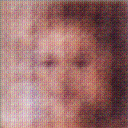
\includegraphics[width=150px]{500_fake_images/samples_5_319.png}%
\caption{A Man With A Beard Wearing A Tie And Glasses}%
\end{figure}

%
\end{document}